\chapter{Implementation}
This chapter will explain 


All these actions are accessed by the Genetic Algorithm to maximize a given Cost Function.

\section{Map and Starting Scenario}
The map is Town10 from Carla. It was chosen, because 1. its roads are self contained, 2. its not too big, yet still complex and 3. its supported by Carla and thus visualization looks better.

The Starting Scenario defines the number and type of all actors as well as their position. It needs to be created manually.
Changing the scenario will have a great impact on the Genetic Algorithms performance. For time and complexity reasons, it was thus decided to first stick with one scenario and do all hyperparameter testing there. And finally test the performance for a handfull different scenarios.

\section{Genetic Algorithm}
\todo{explain why pygad was NOT chosen}
For implementing the Genetic Algorithm, DEAP\todo{cite} was chosen. It is a popular tool for accademia \todo{cite 3 examples}.

\todo{dejong talks about dynamic param and why its not good}

\subsection{Encoding}
When implementing a Genetic Algorithm, it is necessary to implement a Encoding that fits to the problem.
\todo{cite what makes an encoding good: eg. simplicity,...}

\subsubsection{Gene}
Genes are the building blocks of a GA.

\subsubsection{Chromosome}
Each Individual has 1 chomosome which consits of a list of genes. Starting out, 2 different encodings came to mind, in both cases, the genes position in the chromosome defined the time an action is set.

\todo{generate images}
Encoding 1 has the idea that each gene stands for 1 time step. Because multiple actors exist in the simulation, a gene thus needs to be a list of actions. This list always has the length of the number of all actors. This means that crossover can only move all actions of a timestep at once, modifing between actions of the same timestep can only be done using mutation.

Encoding 2 has not only the time step encoded in the position, also the actor ID is encoded. This makes a chromosome now much longer than in the previous encoding, whith the eqatuion beeing: number of timesteps * number of actors. Now crossover has more possibilities.

In the chapter \ref{chap:evaluation} these two chromosome types will be compared.

\subsection{Rules}
Often, actions are not possible if specific requirements are not met. The obvious example is that it is not possible to perform the action AbortLaneChange if there is no current LaneChange happening. LaneChange during a LaneChange is not possible as well. Also Pedestrians can not CrossRoad shortly in a Row.
The hypothesis is that implementing Rules that dont allow for these behaviours will reduce the searchspace and will thus make GA converge quicker.

\todo{be carefull, lanechange after lanechange or crossroad after crossroad might be possible if prev did not happen. Good to explain}
\subsection{Cost Function}
Cost function is a bit difficult, as we are only using interal values. No ADAS/AD system is tested and we thus have to work with what we got.
Currently 3 different cost functions are tested

\subsubsection{Oracles}
While not implemented here, Oracles are needed in order to get a list of good scenarios.


\section{Behavior Tree}
The Behavior Tree will controll the ego vehicle 

\begin{figure}[H]
	\centering
	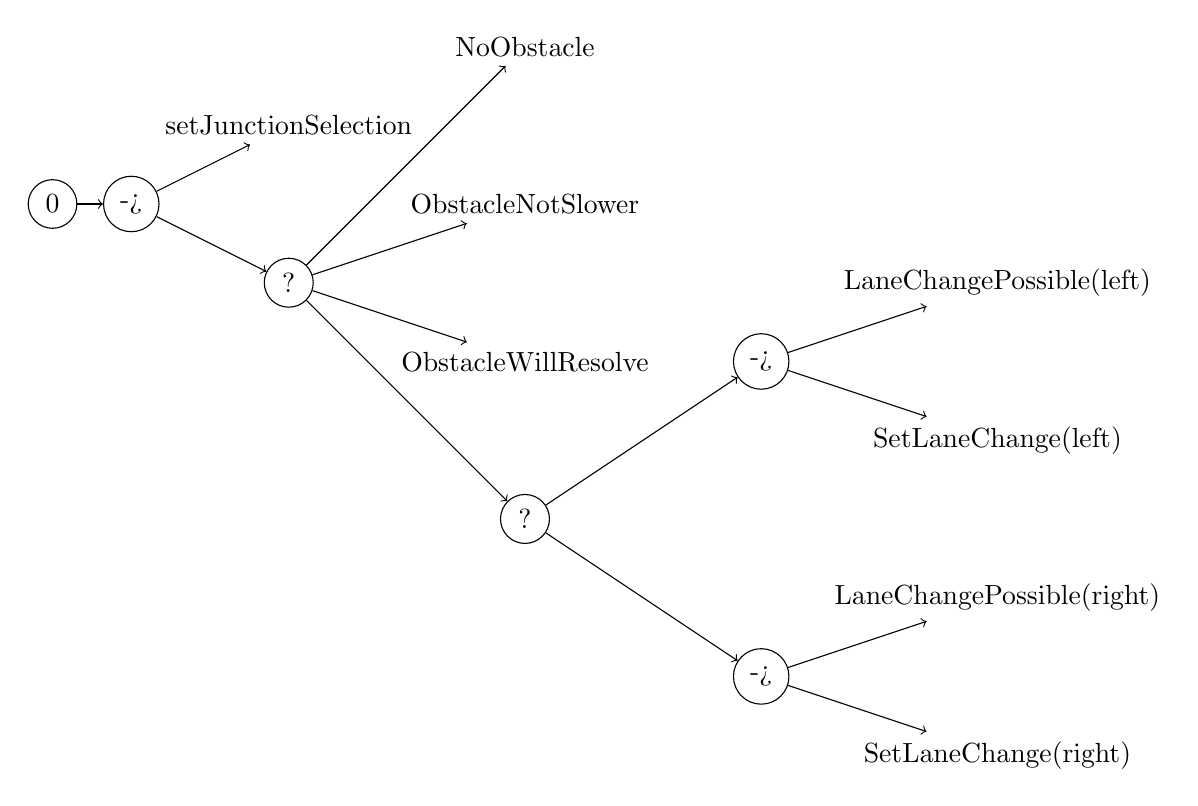
\begin{tikzpicture}
		% Define 1 2 3
		\node[draw, circle] (NodeStart) at (0,0) {0};
		\node[draw, circle] (Sequence1) at (1,0) {->};
		\draw[->] (NodeStart) -- (Sequence1);
		
		\node (Action1) at (3,1) {setJunctionSelection};
		\node[draw, circle] (OR1) at (3,-1) {?};
		\draw[->] (Sequence1) -- (Action1);
		\draw[->] (Sequence1) -- (OR1);

		\node (Action21) at (6,2) {NoObstacle};
		\node (Action22) at (6,0) {ObstacleNotSlower};
		\node (Action23) at (6,-2) {ObstacleWillResolve};
		\node[draw, circle] (OR2) at (6,-4) {?};
		\draw[->] (OR1) -- (Action21);
		\draw[->] (OR1) -- (Action22);
		\draw[->] (OR1) -- (Action23);
		\draw[->] (OR1) -- (OR2);
		
		\node[draw, circle] (Sequence31) at (9,-2) {->};
		\node[draw, circle] (Sequence32) at (9,-6) {->};
		\draw[->] (OR2) -- (Sequence31);
		\draw[->] (OR2) -- (Sequence32);
		
		\node (Action41) at (12,-1) {LaneChangePossible(left)};
		\node (Action42) at (12,-3) {SetLaneChange(left)};
		\node (Action43) at (12,-5) {LaneChangePossible(right)};
		\node (Action44) at (12,-7) {SetLaneChange(right)};
		\draw[->] (Sequence31) -- (Action41);
		\draw[->] (Sequence31) -- (Action42);
		\draw[->] (Sequence32) -- (Action43);
		\draw[->] (Sequence32) -- (Action44);
		
		
	\end{tikzpicture}
	\caption{Used Behaviour Tree}
\end{figure}




